\documentclass{beamer}

\usetheme{Warsaw}
\beamertemplatenavigationsymbolsempty
\boldmath

\usepackage{adjustbox}
\usepackage{graphicx}
\usepackage{url}
\graphicspath{ {./images/} }

\title[Implementation of a Constructive Neural Network]{Design, Implementation and Testing of a Constructive Neural Network Algorithm}
\author[Andrea Orru]{\textbf{Andrea Orru} \small{(ID: 1473018)} \\ \small{Supervisor: Michael Spratling}}
\institute[King's College London]{Department of Informatics \\ King's College London}
\date{2014/2015}
\subject{MSc Intelligent Systems}

\AtBeginSection[]
{
	\begin{frame}
		\frametitle{Table of Contents}
		\tableofcontents[currentsection]
	\end{frame}
}

\begin{document}
	\frame{\titlepage}
	
	\section{Introduction}
		\subsection{Problem and motivation}
			\begin{frame}
				\frametitle{Problem and motivation}
				\framesubtitle{Artificial Neural Networks}
				\begin{block}{Artificial Neural Networks}
					\emph{Artificial neural networks} are a powerful model in machine learning. In theory, an adequately large network is an \emph{universal approximator}.
				\end{block}
				\begin{figure}[h]
					\centering
					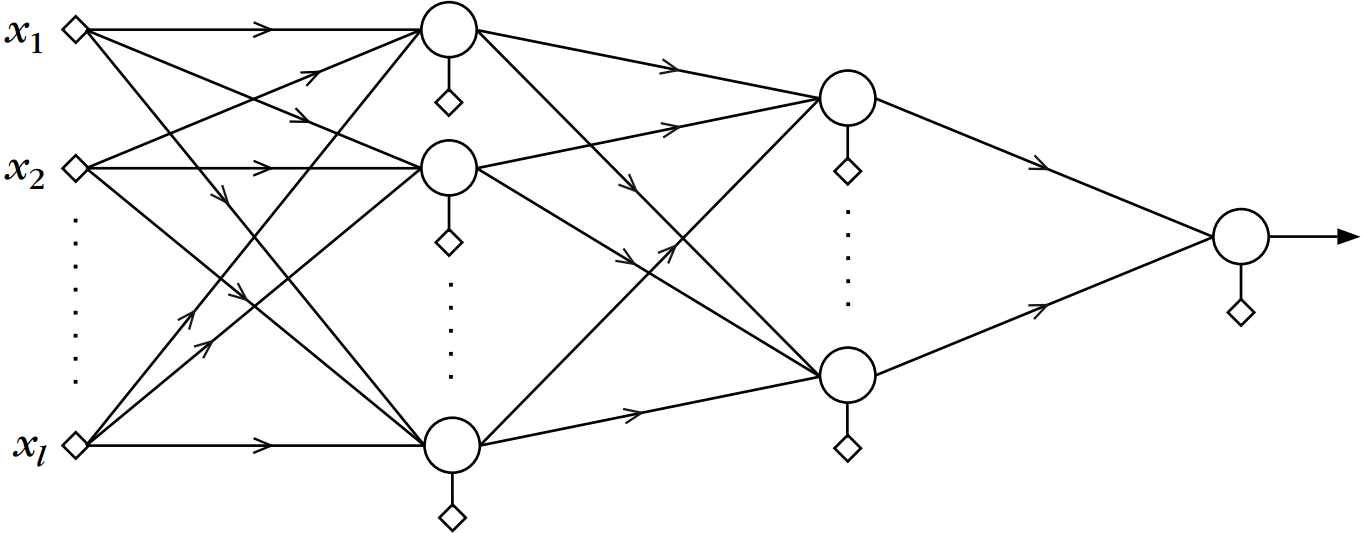
\includegraphics[width=0.65\textwidth]{multilayer}
				\end{figure}
				\begin{alertblock}{Topology}
					In practice, \textbf{too small} networks are unable to learn the problem, while \textbf{overly large} ones tend to \emph{overfit} the training data.
				\end{alertblock}
			\end{frame}
			
			\begin{frame}
				\frametitle{Problem and motivation}
				\framesubtitle{Choosing the topology}
				\begin{block}{Trial and error}
					The architecture of the network is often determined by \emph{trial and error} based on previous experience.
				\end{block}
				\begin{block}{Learning the topology}
					An interesting alternative is \textbf{discovering the topology} as part of the learning algorithm.
				\end{block}
				\begin{exampleblock}{Constructive Neural Network}
					Algorithms that starts from a minimal architecture and then add nodes, connections and layers are called \textbf{\emph{constructive}}.
				\end{exampleblock}
			\end{frame}
			
			\begin{frame}
				\frametitle{Problem and motivation}
				\framesubtitle{Problem definition}
				\begin{exampleblock}{The problem}
					In this project I developed a \textbf{constructive version} of the existing \emph{Divisive Input Modulation} algorithm.
				\end{exampleblock}
				\begin{block}{Why?}
					Small network are \textbf{faster} and \textbf{generalize} better.
				\end{block}
				\begin{block}{Divisive Input Modulation}
					DIM is an unsupervised training algorithm that has \emph{state-of-the-art} performances in \textbf{image decomposition}.
				\end{block}
			\end{frame}
		
		
		\subsection{Background}
			\begin{frame}
				\frametitle{Image decomposition}
				\begin{block}{Image decomposition}
					Finding the \textbf{basic components} from which a set of images are formed, e.g. as a non-negative linear combination of features.
				\end{block}
				\begin{figure}[h]
					\centering
					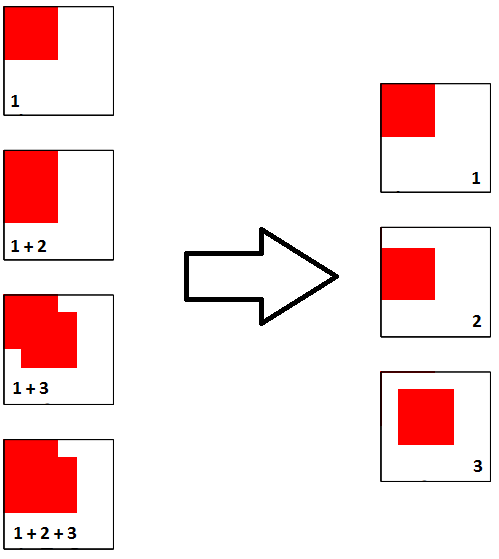
\includegraphics[width=0.43\textwidth]{decomposition}
				\end{figure}
			\end{frame}
			
			\begin{frame}
				\frametitle{Divisive Input Modulation}  
				\begin{columns}[c]
				    \column{0.2\textwidth}
						\begin{figure}[h]
							\centering
							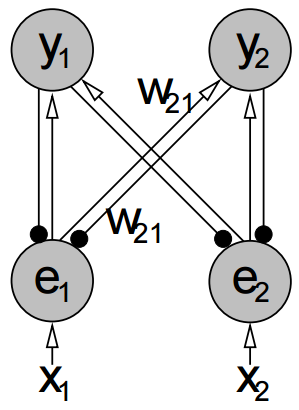
\includegraphics[width=\textwidth]{dim}
						\end{figure}
				    \column{0.8\textwidth}
					    \begin{block}{Inhibitory feedback}
					    	Activation from \emph{predictive} nodes $y_1 ... y_n$ is \textbf{fed back} to \emph{error-detecting} neurons $e_1 ... e_m$ which \emph{modulate} the inputs $x_1 ... x_m$, implementing \emph{competition}.
					    \end{block}
					    \begin{block}{Generative interpretation}
					    	\small{\begin{itemize}
					    		\item $e$: divisive measure of the error ($e_i = 1$ means perfect reconstruction);
					    		\item $W$: row $W_j$ of matrix contains weights to/from neuron $y_j$ and represents a \emph{basic component}.
					    		\item $y$: activation $y_j$ represents the importance of component $j$ in reconstruction of image $x_1 ... x_m$.
					    	\end{itemize}}
					    \end{block}
				\end{columns}
			\end{frame}
		
		
	\section{Implemented algorithm}
		\subsection{Analysis}
			\begin{frame}
				\frametitle{Analysis}
				\framesubtitle{Target of the algorithm}
				\begin{columns}[c]
					\column{0.28\textwidth}
						\begin{figure}[h]
							\centering
							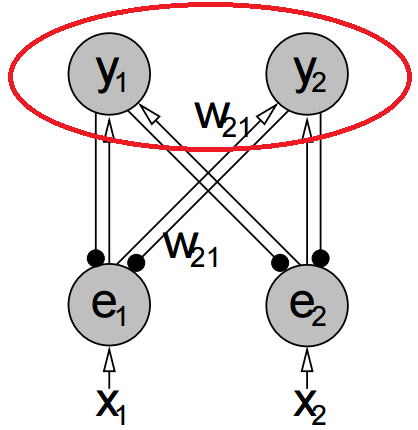
\includegraphics[width=\textwidth]{dim_predictive}
						\end{figure}
					\column{0.8\textwidth}
						\begin{block}{What to grow?}
							The parameter that has to be tuned is $n$, that is, the number of \emph{output/predictive} nodes, and number of rows in the matrix of weights $W$.
						\end{block}
						\begin{exampleblock}{Generative interpretation}
							Parameter $n$ ought to be no less than, and as close as possible to, the number of \emph{\textbf{elementary components}} that form the images in the training set.
						\end{exampleblock}
				\end{columns}
			\end{frame}
		
			\begin{frame}
				\frametitle{Analysis}
				\framesubtitle{Measure of performance of the network}
				\begin{columns}[c]
					\column{0.28\textwidth}
					\begin{figure}[h]
						\centering
						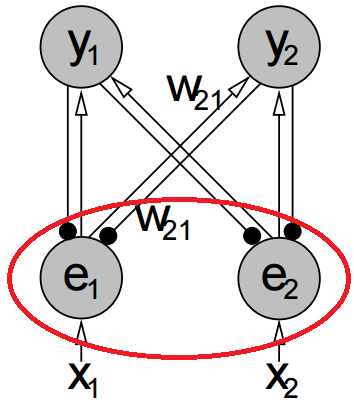
\includegraphics[width=\textwidth]{dim_error}
					\end{figure}
					\column{0.8\textwidth}
					\begin{exampleblock}{Generative interpretation}
						Error-detecting nodes provide an estimation of the accuracy of the reconstruction. Perfect representation of pixel $x_i$ is achieved when $e_i = 1$.
					\end{exampleblock}
					\begin{block}{Error of the network}
						Criteria based on the distance $\left|e_i - 1\right|$ across the whole image and all the images in the training set can be used to take decisions over the size of the network.
					\end{block}
				\end{columns}
			\end{frame}
		
		
		\subsection{Design}
			\begin{frame}
				\frametitle{Design}
				\framesubtitle{Criteria for growing the network}
				\begin{block}{When to grow?}
					Intuitively, if the rate of change of the error during learning stays below a \emph{\textbf{trigger slope}} $\Delta_T$ for too long, the network is unlikely to improve significantly any more, so new nodes are needed.
				\end{block}
				\begin{figure}[h]
					\centering
					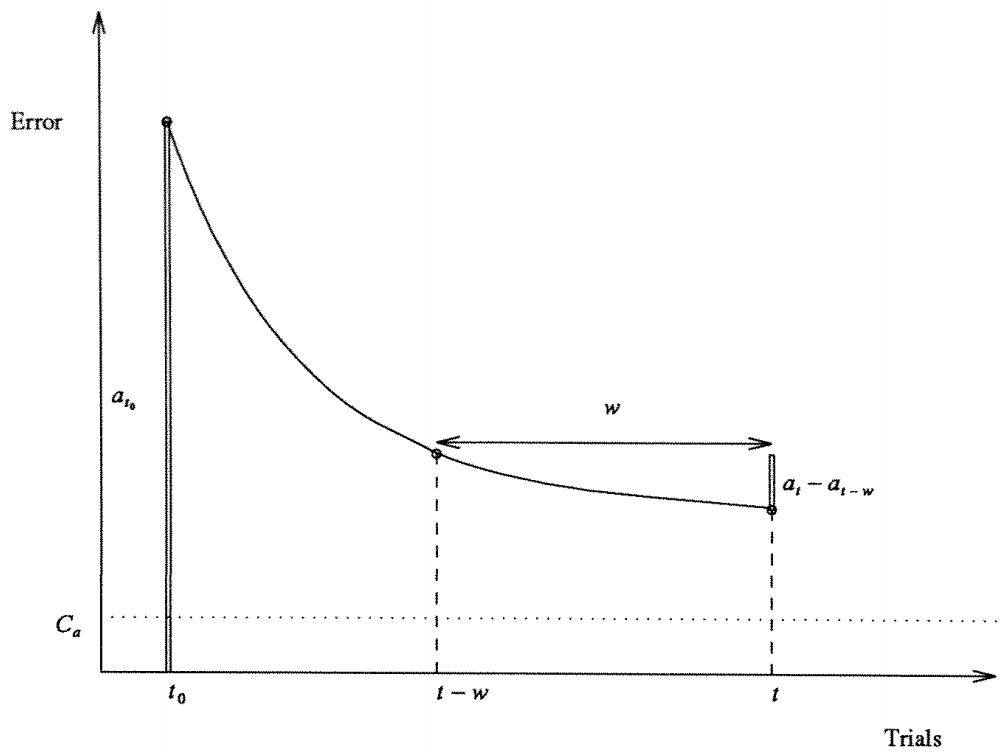
\includegraphics[width=0.56\textwidth]{error}
				\end{figure}
			\end{frame}

			\begin{frame}
				\frametitle{Design}
				\framesubtitle{Criteria for growing the network (continued)}
				\begin{block}{Growth}
					A certain number of nodes (by default 1) is added to the network when the network struggles to improve.
				\end{block}
				\begin{exampleblock}{Exponential growth}
					If the error is very high (over a threshold $C_e$), the number of neurons is increased by a multiplicative factor.
				\end{exampleblock}
				\begin{alertblock}{Stopping criteria}
					To stop the network from growing indefinitely, a parameter $C_s$ is set. If the error of the network ever goes under this threshold, the size of the network will not change any more.
				\end{alertblock}
			\end{frame}

			\begin{frame}
				\frametitle{Design}
				\framesubtitle{Weight (re)training}
				\begin{block}{Full retraining}
					Every time the network changes topology, all the weights are retrained.
				\end{block}
				\begin{block}{Weight freezing}
					When a node is added to the network, the existing weights are preserved and only the new ones are trained.
				\end{block}
				\begin{exampleblock}{Rationale for my choice}
					Even though weight freezing is faster, it allows to find solutions only in an \emph{affine subset} of the weight space. \textbf{Full retraining} produces more accurate results.
				\end{exampleblock}
			\end{frame}


		\subsection{Results}
			\begin{frame}
				\frametitle{Benchmarks}
				\framesubtitle{Squares problem}
				\begin{itemize}
					\item Each image is generated by randomly selecting an element from a set of $s \times s$ pixel squares.
					\item Each component has a \emph{probability} of appearance, a \emph{contrast} and a \emph{depth}.
					\item Each pixel in the image gets assigned the contrast of the foremost square in that location, if any.
				\end{itemize}
				\begin{figure}[h]
					\centering
					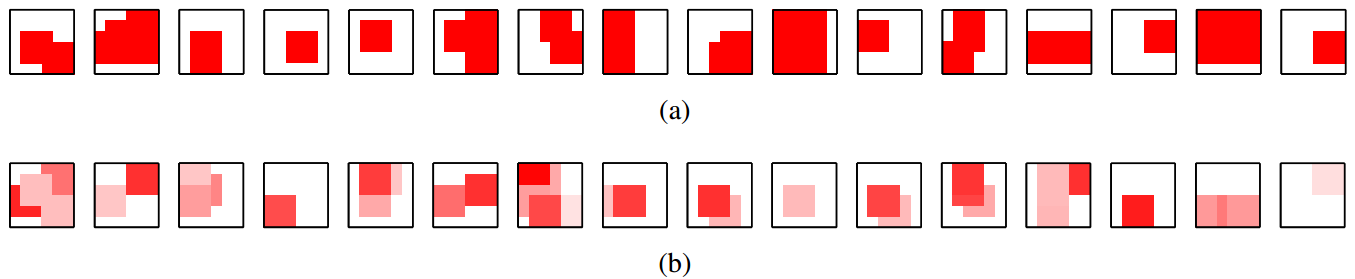
\includegraphics[width=\textwidth]{squares}
				\end{figure}
			\end{frame}
			
			\begin{frame}
				\frametitle{Constructive DIM}
				\framesubtitle{Squares problem}
\begin{table}[h]
	\centering
	\begin{adjustbox}{width=1\textwidth}
		\begin{tabular}{l*{4}{|c}}
			\emph{Algorithm}          & \emph{Accuracy}  & \emph{Cycles}            & \emph{Training time}     & \emph{Nodes}                       \\
			\hline
			DIM (32 nodes)            & 98.01\%          & 20000 (fixed)            & 11.50s (average)         & 32 (fixed)                         \\
			\textbf{Constructive DIM} & \textbf{97.94\%} & \textbf{21720 (average)} & \textbf{8.23s (average)} & \textbf{22.66 (average)}           \\
			DIM (time-constrained)    & 96.19\%          & 19911 (average)          & 8.23s (constrained)      & $\lceil$22.66$\rceil$ = 23 (fixed) \\
			DIM (16 nodes)            & 89.31\%          & 20000 (fixed)            & 6.15s (average)         & 16 (fixed)                          \\
		\end{tabular}
	\end{adjustbox}
\end{table}
				\begin{columns}[c]
					\column{0.7\textwidth}
						\begin{small}
							\begin{itemize}
								\item 16 real components.
								\item \textbf{Constructive DIM} was almost as accurate as a 32 nodes DIM network, while being \textbf{\url{~}40\% faster} and using \textbf{22.66 nodes} on average.
								\item DIM running on the same conditions (fixed execution time and 23 nodes) performed slightly worse than Constructive DIM.
							\end{itemize}
						\end{small}
					\column{0.4\textwidth}	
						\begin{figure}[h]
							\centering
							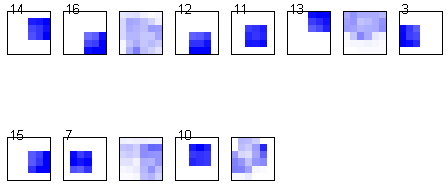
\includegraphics[width=\textwidth]{learning_squares}
						\end{figure}
				\end{columns}
			\end{frame}
			
			
	\section{Conclusions}
		\begin{frame}
			\frametitle{Conclusions}
			\begin{block}{What was done}
				I developed a \textbf{constructive version} of the \emph{state-of-the-art} DIM algorithm, which automatically evolves the network to an adequate size during learning.
			\end{block}
			\begin{block}{Results}
				The resulting algorithm has the same level of accuracy, but it is faster and produces small networks.
			\end{block}
		\end{frame}
\end{document}